\documentclass[graphics]{beamer}

\usepackage{graphicx}
\usepackage{verbatim}
\usepackage{wrapfig}
\useoutertheme{shadow}
%\usecolortheme{orchid}
\usecolortheme{seahorse}


% math commands
\newcommand{\be}{\begin{eqnarray}}
\newcommand{\ee}{\end{eqnarray}}
\newcommand{\beq}{\begin{equation}}
\newcommand{\eeq}{\end{equation}}
\def\simless{\mathbin{\lower 3pt\hbox
      {$\rlap{\raise 5pt\hbox{$\char'074$}}\mathchar"7218$}}}
\def\simgreat{\mathbin{\lower 3pt\hbox
      {$\rlap{\raise 5pt\hbox{$\char'076$}}\mathchar"7218$}}} %> or of order

% variables

\def\toonscale{0.45}
\def\mboxy#1{\mbox{\small #1}}


\begin{comment}
\AtBeginSection[]{
  \frame{
    \frametitle{Outline}
    \tableofcontents[currentsection]
  }
}
\end{comment}

\title{Directional Spin
}
\subtitle{}
\author[U. Pen]{\textcolor{green}{Ue-Li Pen, Pavel Motloch, Haoran Yu}
\\[8mm] 
}
\date{February 27, 2020}


\begin{document}

\frame{
\begin{picture}(320,250)
\put(-50,-130){
\includegraphics[width=5.7in]{Figures/delta_nu_sim.pdf}}
\end{picture}
\vspace{-3in}
\titlepage
}

%\section*{Introduction}
\section{Directional Spin}

\begin{comment}
  \subsection{Outline}

  \frame{
    \frametitle{Outline}
    \tableofcontents
  }
\end{comment}


  \frame{
    \frametitle{Introduction}
    \begin{itemize}
    \item Lagrangian vs Eulerian: LSS is much simpler in Lagrangian
      space
    \item Reconstruction: solving for Lagrangian coordinates
    \item Towards the beginning: initial tidal shear
    \item Galaxy spins are fossils of small scale IC
    \item Simulations: angular momentum directions of TTT, DM,
      Baryons very well aligned, readily observables.  Magnitudes poorly predicted, and
          not observable.
        \item previous studies mostly focussed on weak, residual alignments
        \item New: measuring and predicting {\it oriented} spin
        \end{itemize}
}


\frame{
    \frametitle{Inference}
\includegraphics[width=4.1in]{Figures/alignment.pdf}  
  }



\frame{
    \frametitle{Zoo}
\includegraphics[width=4.1in]{Figures/land2008.png}  
  }


\frame{
    \frametitle{Prograde Winding}
\includegraphics[width=3.1in]{Figures/fantomm.png}  

(NGC6946, from Fathi+ 2007)
  }
%\frame{
 %   \frametitle{Tilt}
%\includegraphics[width=4.1in]{Figures/SAMI.png}  
%(SAMI, 1409.4147)
 % }


  \frame{
    \frametitle{Observables}
    \begin{itemize}
      \item 3-D position (redshift)
        \item ellipticity
        \item position angle
        \item winding direction (S vs Z)
        \item reddening
        \item human and machine classifications for $10^{4-6}$ objects
          (galaxy zoo, Land+ 2008 )
    \end{itemize}
}

  \frame{
    \frametitle{Galaxy Spins}
    \begin{itemize}
        \item most galaxies are rotating disks of stars and gas
        \item readily identifyable spin axis
        \item trailing spiral arms, (HI) velocity
          (rotation) field, (dust lanes)
        \item largest sample from galaxy zoo (13546 $\hat{j}_\parallel$),
          SAMI/MaNGA (1609 $\hat{j}_\perp$), 600 full spin vector $\hat{j}$
        \item new result (Motloch et al 2020): 3.4$\sigma$ oriented
          direction correlation with ELUCID reconstructed tide and
          inertia field
     \end{itemize}
}

\frame{
    \frametitle{Tidal Torque}
\includegraphics[width=6.1in]{Figures/protospin.pdf}  
  }


\frame{
    \frametitle{Simulation Lagrangian Correlation}
\vspace{-0.1in}
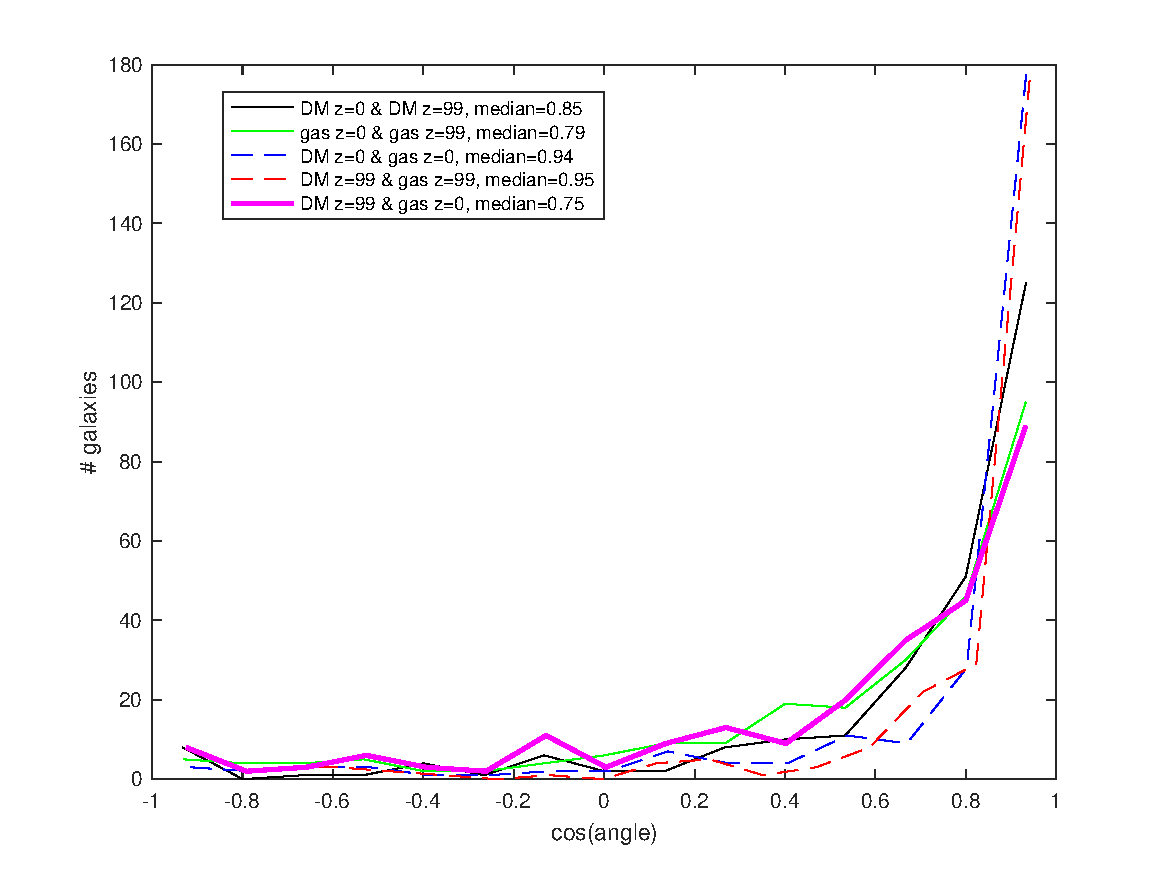
\includegraphics[width=4.0in]{Figures/Illustris_Lagrangian_AM_cosangle_distributions_allgas.pdf}  

Noise smaller than Poisson! (Illustris, from Shy Genel)
  }

  \frame{
    \frametitle{Context}
    \begin{itemize}
    \item prehistory: Hoyle 1949, Peebles 1969
        \item S White 1984: TTT
        \item Lee\&Pen 2000: LSS statistical theory
        \item Yu++ 2018: Lagrangian theory, high fidelity direction
          memory, poor magnitude memory
        \item Genel++: spin magnitude
     \end{itemize}
}


  \frame{
    \frametitle{Angular momentum}
    \begin{itemize}
        \item 1st order effect from misalignment of moment of inertia
          and tidal tensor
        \item torque: $\tau\equiv\int \rho \bf{r} \times \nabla \phi$
        \item Taylor expand: $\tau_i=\epsilon_{ijk} \int \rho x^jx^l \partial_l\partial_k\phi \equiv\epsilon_{ijk} I_{il}T_{lk}$
        \item Tensor form $\tau= * I \cdot T$
        \item first realized by S.D.M. White (1984), see also LP00
        \item $T$ and $\hat{\tau}$ observable -- what about $I$?
     \end{itemize}
}

\frame{
    \frametitle{E-mode: Origami}

\hspace{-0.2in}\includegraphics[width=2.3in]{Figures/nonlinear.png}  
\vspace{0.15in}\includegraphics[width=2.21in]{Figures/reconstructed.png}  

Eulerian (L) vs Lagrangian (R) (from Yu et al 2016, 1610.7112,
originally Neyrinck+ 2012)
  }

  \frame{
    \frametitle{Tensors}
    \begin{itemize}
        \item Tide: ${\bf T}$ reconstructed from density field
        \item Inertia: non-linear reconstruction of ${\bf I}$
        \item strongly correlated
     \end{itemize}
}
\frame{
    \frametitle{Sim}
\includegraphics[width=4.1in]{Figures/I-T.png}  
Yu+2018
  }

\frame{
    \frametitle{Lagrangian coordinates}
\center{\includegraphics[width=4.3in]{Figures/delta_reco_raw.pdf}  }
  }
\frame{
\vspace{-0.5in}
    \frametitle{Reconstruction}
    \begin{itemize}
        \item multiple successful approaches
        \item injective Isobaric (Pen++ 1995, Zhu/Wang/Yu/ 2016-2020 )
        \item ELUCID, Schmidtful17,  Shi18, Hada18, Hikage19, etc
        \item typically achieve 50\% phase fidelity per mode up to
          $k\sim 1h$/Mpc in simulations
        \item up to $\sim$ 3/h Mpc for SDSS sampling density in ELUCID
     \end{itemize}
  }
\frame{
\vspace{-0.5in}
    \frametitle{What about Inertia Tensor?}
    \begin{itemize}
        \item {\bf I} readily measured in simulations
        \item highly correlated with tide {\bf T}
        \item depends on small misalignment with {\it external} shear
        \item use small scale tide as proxy for inertia, and larger
          scale for tide
        \item Taylor expansion: {\bf I}$_{ab}=\partial_a\partial_b\rho$
        \item in progress: Lagrangian space tesselation?
     \end{itemize}
  }

\frame{
    \frametitle{Current Status}
\includegraphics[width=3.1in]{Figures/zoohist.png}  
{\tiny Motloch, Yu, ULP 2020}
  }

\frame{
%\vspace{-0.5in}
    \frametitle{Conclusions}
    \begin{itemize}
      \item Galaxy spin oriented direction well determined by
        Lagrangian cosmic structure: Tide and Inertia
      \item Partially reconstructable from non-linear cosmic web: two
        scale tensors, {\bf I} and {\bf T}
      \item oriented direction readily observed and well preserved in
        non-linear (baryonic) evolution
      \item Initial detection in ELUCID-zoo-IFU comparison
          \item parity odd field, less likely to be contaminated
            (e.g. lensing)
          \item limited by small scale initial density field: benefit
            from reconstruction with 21cm IM?
          \item potentially access to very large number ($10^{11}$?)
            of small scale modes in early universe.  Parity/helicity,
            neutrinos, $f_{NL}$, GW, etc.
     \end{itemize}
  }


\end{document}
